\section{Diagrama de estados}

Nesta secção, apresentamos o diagrama de estado do nosso sistema (figura \ref{fig:diagrama_de_estado}).

\begin{figure}[h]
    \centering
    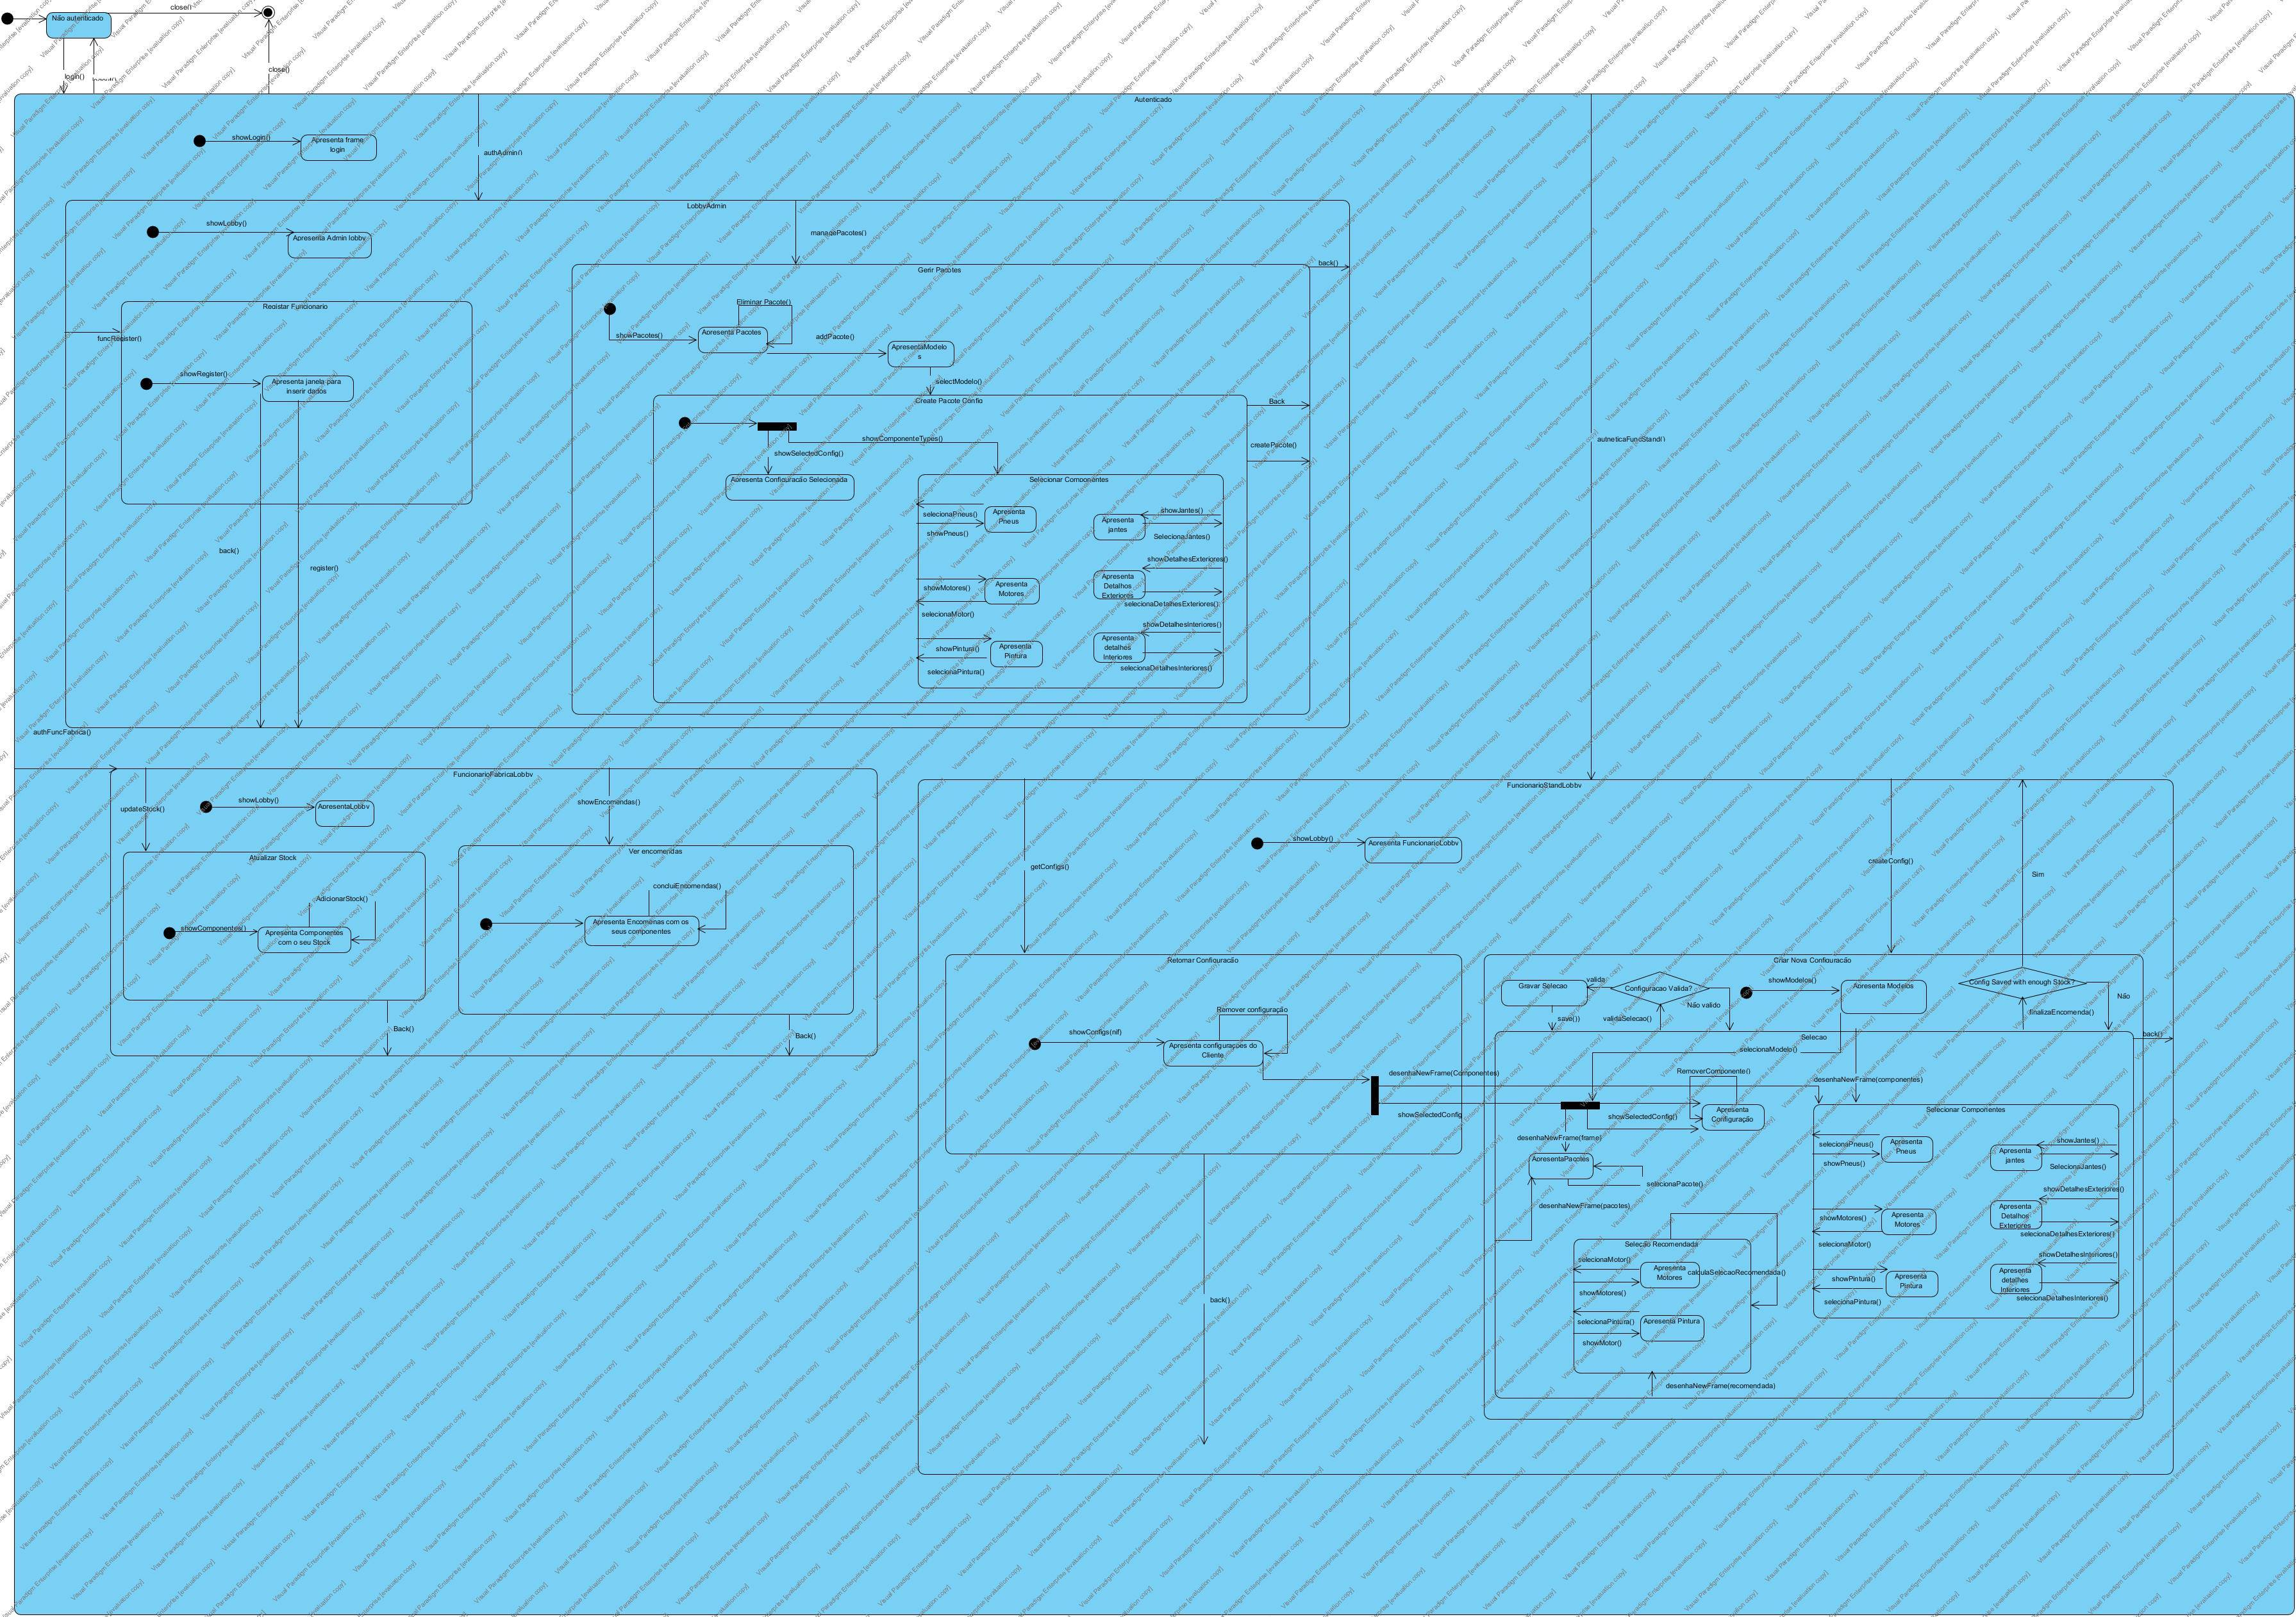
\includegraphics[width=\textwidth]{analise_de_requisitos/49461754_398655354223097_8464874533138989056_n.jpg}
    \caption{Diagrama de estado}
    \label{fig:diagrama_de_estado}
\end{figure}


Neste diagrama, admitimos que existe um superestado chamado “autenticado”, que surge quando se efetua o \textit{login}. Este estado direciona o utilizador para diferentes subestados, dependendo da sua função no sistema. Se o utilizador for um funcionário de fábrica, este tem acesso ao métodos representados no lado esquerdo do modelo acima, que correspondem à atualização do stock (jantes, motores, pintura e pneus). Se o utilizador for um administrador, só tem acesso aos métodos que lhe permitem registar funcionários e criar/eliminar pacotes do sistema. Por último, todos os funcionários de stand têm acesso às funcionalidades faladas já nas secções anteriores, que estão representadas no lado direito do superestado do diagrama (fig. \ref{fig:diagrama_de_estado}).


\clearpage